\documentclass[10pt,a4paper,landscape]{article}
\usepackage[margin=0.5cm]{geometry}
\usepackage{multicol}
\usepackage{amsmath,amssymb}
\usepackage{enumitem}
\usepackage{tikz}
\usetikzlibrary{shapes,arrows}

\setlength{\columnseprule}{0.4pt}
\setlist{nosep}
\pagestyle{empty}

\tikzstyle{startstop} = [rectangle, rounded corners, minimum width=3cm, minimum height=1cm, text centered, draw=black]
\tikzstyle{process} = [rectangle, minimum width=3cm, minimum height=1cm, text centered, draw=black]
\tikzstyle{decision} = [diamond, minimum width=3cm, minimum height=1cm, text centered, draw=black]
\tikzstyle{arrow} = [thick,->,>=stealth]

\begin{document}

% Page 1
\begin{multicols}{2}

\section*{Basic Concepts and Linear Algebra}

\subsection*{Optimization Problem Standard Form}
\begin{align}
\min/\max \quad & f(x) \\
\text{s.t.} \quad & g_i(x) \leq b_i \quad \text{(inequality constraints)} \\
& h_j(x) = c_j \quad \text{(equality constraints)} \\
& x \in X \quad \text{(variable bounds)}
\end{align}

\subsection*{Linear Algebra Fundamentals}
\begin{itemize}
\item \textbf{Rank}: Maximum number of linearly independent rows/columns
\item \textbf{Matrix multiplication}: $C = AB$, $c_{ij} = \sum_k a_{ik}b_{kj}$
\item \textbf{Matrix inverse}: $AA^{-1} = I$
\item \textbf{System of equations} $Ax = b$:
  \begin{itemize}
  \item $m = n$, $\text{rank}(A) = n \rightarrow$ unique solution
  \item $m < n \rightarrow$ infinite solutions
  \item $\text{rank}(A) < \text{rank}([A|b]) \rightarrow$ no solution
  \end{itemize}
\end{itemize}

\subsection*{Gradient and Hessian}
\begin{itemize}
\item \textbf{Gradient}: $\nabla f(x) = \begin{bmatrix} \frac{\partial f}{\partial x_1} \\ \vdots \\ \frac{\partial f}{\partial x_n} \end{bmatrix}$
\item \textbf{Hessian}: $\nabla^2 f(x) = \left[\frac{\partial^2 f}{\partial x_i \partial x_j}\right]$
\item \textbf{1st order Taylor}: $f(x) \approx f(x_0) + \nabla f(x_0)^T(x - x_0)$
\item \textbf{2nd order Taylor}: $f(x) \approx f(x_0) + \nabla f(x_0)^T(x - x_0) + \frac{1}{2}(x - x_0)^T\nabla^2 f(x_0)(x - x_0)$
\end{itemize}

\subsection*{Optimality Conditions}
\begin{itemize}
\item \textbf{First-order necessary}: $\nabla f(x^*) = 0$
\item \textbf{Second-order sufficient}: 
  \begin{itemize}
  \item min problem: $\nabla^2 f(x^*)$ positive definite (PD)
  \item max problem: $\nabla^2 f(x^*)$ negative definite (ND)
  \end{itemize}
\end{itemize}

\columnbreak

\section*{Convexity Decision Flowchart}

\subsection*{Convex Set Decision}
\begin{center}
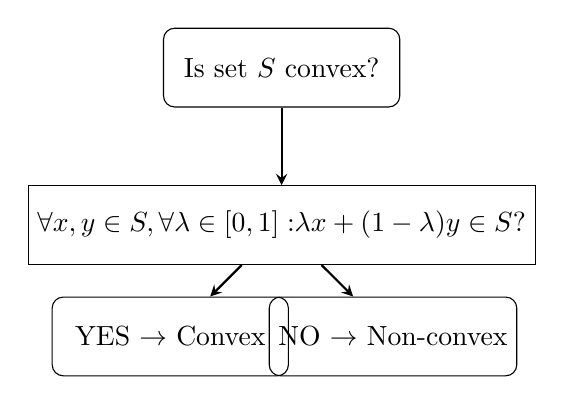
\begin{tikzpicture}[node distance=2cm]
\node (start) [startstop] {Is set $S$ convex?};
\node (test) [process, below of=start] {$\forall x,y \in S, \forall \lambda \in [0,1]:$ \\ $\lambda x + (1-\lambda)y \in S$?};
\node (yes) [startstop, below left of=test] {YES $\rightarrow$ Convex};
\node (no) [startstop, below right of=test] {NO $\rightarrow$ Non-convex};

\draw [arrow] (start) -- (test);
\draw [arrow] (test) -- (yes);
\draw [arrow] (test) -- (no);
\end{tikzpicture}
\end{center}

\textbf{Examples of Convex Sets}:
\begin{itemize}
\item Hyperplane: $\{x | a^T x = b\}$
\item Halfspace: $\{x | a^T x \leq b\}$
\item Ball: $\{x | \|x - c\| \leq r\}$
\item Polyhedron: $Ax \leq b$
\end{itemize}

\subsection*{Convex Function Decision}
\begin{center}
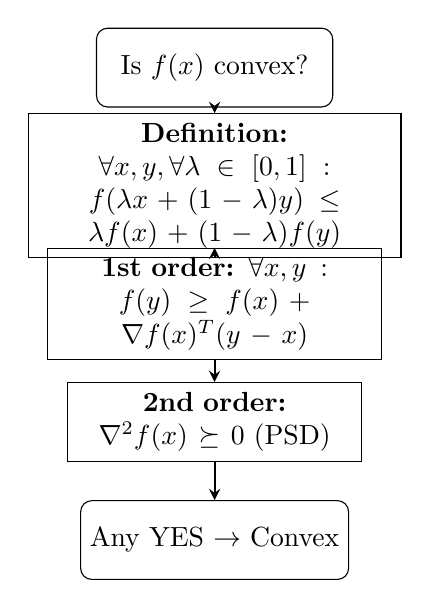
\begin{tikzpicture}[node distance=1.5cm]
\node (start) [startstop] {Is $f(x)$ convex?};
\node (def) [process, below of=start, text width=4.5cm] {\textbf{Definition:} $\forall x,y, \forall \lambda \in [0,1]:$ \\ $f(\lambda x + (1-\lambda)y) \leq \lambda f(x) + (1-\lambda)f(y)$};
\node (first) [process, below of=def, text width=4cm] {\textbf{1st order:} $\forall x,y:$ \\ $f(y) \geq f(x) + \nabla f(x)^T(y - x)$};
\node (second) [process, below of=first, text width=3.5cm] {\textbf{2nd order:} \\ $\nabla^2 f(x) \succeq 0$ (PSD)};
\node (result) [startstop, below of=second] {Any YES $\rightarrow$ Convex};

\draw [arrow] (start) -- (def);
\draw [arrow] (def) -- (first);
\draw [arrow] (first) -- (second);
\draw [arrow] (second) -- (result);
\end{tikzpicture}
\end{center}

\textbf{PSD Test Methods}:
\begin{itemize}
\item All eigenvalues $\geq 0$
\item Leading principal minors $\geq 0$
\item $x^T A x \geq 0 \, \forall x$
\end{itemize}

\end{multicols}

\newpage

% Page 2
\begin{multicols}{2}

\section*{Convex Programming and Linear Programming}

\subsection*{Convex Programming Decision}
\begin{center}
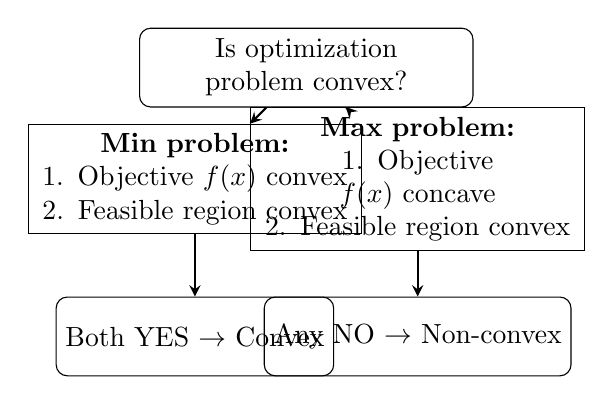
\begin{tikzpicture}[node distance=2cm]
\node (start) [startstop, text width=4cm] {Is optimization problem convex?};
\node (min) [process, below left of=start, text width=4cm] {\textbf{Min problem:} \\ 1. Objective $f(x)$ convex \\ 2. Feasible region convex};
\node (max) [process, below right of=start, text width=4cm] {\textbf{Max problem:} \\ 1. Objective $f(x)$ concave \\ 2. Feasible region convex};
\node (result1) [startstop, below of=min] {Both YES $\rightarrow$ Convex};
\node (result2) [startstop, below of=max] {Any NO $\rightarrow$ Non-convex};

\draw [arrow] (start) -- (min);
\draw [arrow] (start) -- (max);
\draw [arrow] (min) -- (result1);
\draw [arrow] (max) -- (result2);
\end{tikzpicture}
\end{center}

\subsection*{Linear Programming}
\textbf{Standard Form}:
\begin{align}
\min \quad & c^T x \\
\text{s.t.} \quad & Ax = b \\
& x \geq 0
\end{align}

\textbf{Key Terms}:
\begin{itemize}
\item \textbf{Basic solution}: Solution with $n$ basic variables
\item \textbf{Basic feasible solution (BFS)}: Basic + feasible
\item \textbf{Degeneracy}: Basic variable = 0
\item \textbf{Extreme point}: Vertex of polyhedron
\item \textbf{Extreme ray}: Unbounded direction
\end{itemize}

\subsection*{Simplex Method Steps}
\begin{enumerate}
\item Find \textbf{initial BFS}
\item \textbf{Optimality test}: Reduced costs $\leq 0$
\item \textbf{Direction}: Choose entering variable
\item \textbf{Step size}: Minimum ratio test
\item \textbf{Update basis}: Choose leaving variable
\end{enumerate}

\columnbreak

\section*{Special Problems and Practical Formulas}

\subsection*{Transportation Problem}
\begin{align}
\min \quad & \sum_i \sum_j c_{ij} x_{ij} \\
\text{s.t.} \quad & \sum_j x_{ij} \leq s_i \quad \text{(supply)} \\
& \sum_i x_{ij} \geq d_j \quad \text{(demand)} \\
& x_{ij} \geq 0
\end{align}

\textbf{Infeasibility}: $\sum s_i < \max\{d_j\}$

\subsection*{Absolute Value Linearization}
\begin{align}
\min |x - a| \quad \rightarrow \quad & \min z \\
\text{s.t.} \quad & z \geq x - a \\
& z \geq -(x - a)
\end{align}

\subsection*{Set Properties}
Set $X = \{x \in [a,b]^n : \sum x_i \geq c\}$
\begin{itemize}
\item \textbf{Bounded}: $[a,b]$ finite intervals
\item \textbf{Closed}: Defined by equalities/inequalities
\item \textbf{Convex}: Intersection of box + linear constraints
\end{itemize}

\subsection*{Common Convex Functions}
\begin{itemize}
\item $x^k$ ($k \geq 1$, $x \geq 0$): convex
\item $\ln(x)$ ($x > 0$): concave
\item $e^x$: convex
\item $x^2 + y^2$: convex
\item $\max\{f_1(x), f_2(x)\}$: convex if $f_1, f_2$ convex
\item $|x|$: convex
\end{itemize}

\subsection*{Decision Timing}
\begin{itemize}
\item \textbf{Here-and-now}: Decide before uncertainty
\item \textbf{Wait-and-see}: Decide after uncertainty
\end{itemize}

\subsection*{Key Calculations from Past Exams}
\begin{itemize}
\item \textbf{Gradient}: $f(x_1,x_2) = \sqrt{x_1-1} + (x_2-1)^{1/4}$ at $(3,2)$
  \[\nabla f = \begin{bmatrix} \frac{1}{2\sqrt{2}} \\ \frac{1}{4} \end{bmatrix}\]
\item \textbf{Hessian}: $f(x_1,x_2) = 2(x_1-3)^2 + 6x_1x_2 + 2(x_2+3)^2 + 6x_1 + 2x_2$ at $(2,3)$
  \[H = \begin{bmatrix} 4 & 6 \\ 6 & 4 \end{bmatrix}\]
\end{itemize}

\end{multicols}

\vfill

\section*{Important Abbreviations}
\begin{itemize}
\item \textbf{LP}: Linear Programming
\item \textbf{NLP}: Nonlinear Programming  
\item \textbf{BFS}: Basic Feasible Solution
\item \textbf{PSD}: Positive Semidefinite
\item \textbf{PD}: Positive Definite
\item \textbf{s.t.}: subject to
\end{itemize}

\end{document}